% Options for packages loaded elsewhere
\PassOptionsToPackage{unicode}{hyperref}
\PassOptionsToPackage{hyphens}{url}
\PassOptionsToPackage{dvipsnames,svgnames,x11names}{xcolor}
%
\documentclass[
  10pt,
  letterpaper,
  DIV=11,
  numbers=noendperiod]{scrartcl}

\usepackage{amsmath,amssymb}
\usepackage{setspace}
\usepackage{iftex}
\ifPDFTeX
  \usepackage[T1]{fontenc}
  \usepackage[utf8]{inputenc}
  \usepackage{textcomp} % provide euro and other symbols
\else % if luatex or xetex
  \usepackage{unicode-math}
  \defaultfontfeatures{Scale=MatchLowercase}
  \defaultfontfeatures[\rmfamily]{Ligatures=TeX,Scale=1}
\fi
\usepackage{lmodern}
\ifPDFTeX\else  
    % xetex/luatex font selection
  \setmonofont[Scale=0.75]{Source Code Pro}
\fi
% Use upquote if available, for straight quotes in verbatim environments
\IfFileExists{upquote.sty}{\usepackage{upquote}}{}
\IfFileExists{microtype.sty}{% use microtype if available
  \usepackage[]{microtype}
  \UseMicrotypeSet[protrusion]{basicmath} % disable protrusion for tt fonts
}{}
\makeatletter
\@ifundefined{KOMAClassName}{% if non-KOMA class
  \IfFileExists{parskip.sty}{%
    \usepackage{parskip}
  }{% else
    \setlength{\parindent}{0pt}
    \setlength{\parskip}{6pt plus 2pt minus 1pt}}
}{% if KOMA class
  \KOMAoptions{parskip=half}}
\makeatother
\usepackage{xcolor}
\setlength{\emergencystretch}{3em} % prevent overfull lines
\setcounter{secnumdepth}{-\maxdimen} % remove section numbering
% Make \paragraph and \subparagraph free-standing
\ifx\paragraph\undefined\else
  \let\oldparagraph\paragraph
  \renewcommand{\paragraph}[1]{\oldparagraph{#1}\mbox{}}
\fi
\ifx\subparagraph\undefined\else
  \let\oldsubparagraph\subparagraph
  \renewcommand{\subparagraph}[1]{\oldsubparagraph{#1}\mbox{}}
\fi

\usepackage{color}
\usepackage{fancyvrb}
\newcommand{\VerbBar}{|}
\newcommand{\VERB}{\Verb[commandchars=\\\{\}]}
\DefineVerbatimEnvironment{Highlighting}{Verbatim}{commandchars=\\\{\}}
% Add ',fontsize=\small' for more characters per line
\usepackage{framed}
\definecolor{shadecolor}{RGB}{241,243,245}
\newenvironment{Shaded}{\begin{snugshade}}{\end{snugshade}}
\newcommand{\AlertTok}[1]{\textcolor[rgb]{0.68,0.00,0.00}{#1}}
\newcommand{\AnnotationTok}[1]{\textcolor[rgb]{0.37,0.37,0.37}{#1}}
\newcommand{\AttributeTok}[1]{\textcolor[rgb]{0.40,0.45,0.13}{#1}}
\newcommand{\BaseNTok}[1]{\textcolor[rgb]{0.68,0.00,0.00}{#1}}
\newcommand{\BuiltInTok}[1]{\textcolor[rgb]{0.00,0.23,0.31}{#1}}
\newcommand{\CharTok}[1]{\textcolor[rgb]{0.13,0.47,0.30}{#1}}
\newcommand{\CommentTok}[1]{\textcolor[rgb]{0.37,0.37,0.37}{#1}}
\newcommand{\CommentVarTok}[1]{\textcolor[rgb]{0.37,0.37,0.37}{\textit{#1}}}
\newcommand{\ConstantTok}[1]{\textcolor[rgb]{0.56,0.35,0.01}{#1}}
\newcommand{\ControlFlowTok}[1]{\textcolor[rgb]{0.00,0.23,0.31}{#1}}
\newcommand{\DataTypeTok}[1]{\textcolor[rgb]{0.68,0.00,0.00}{#1}}
\newcommand{\DecValTok}[1]{\textcolor[rgb]{0.68,0.00,0.00}{#1}}
\newcommand{\DocumentationTok}[1]{\textcolor[rgb]{0.37,0.37,0.37}{\textit{#1}}}
\newcommand{\ErrorTok}[1]{\textcolor[rgb]{0.68,0.00,0.00}{#1}}
\newcommand{\ExtensionTok}[1]{\textcolor[rgb]{0.00,0.23,0.31}{#1}}
\newcommand{\FloatTok}[1]{\textcolor[rgb]{0.68,0.00,0.00}{#1}}
\newcommand{\FunctionTok}[1]{\textcolor[rgb]{0.28,0.35,0.67}{#1}}
\newcommand{\ImportTok}[1]{\textcolor[rgb]{0.00,0.46,0.62}{#1}}
\newcommand{\InformationTok}[1]{\textcolor[rgb]{0.37,0.37,0.37}{#1}}
\newcommand{\KeywordTok}[1]{\textcolor[rgb]{0.00,0.23,0.31}{#1}}
\newcommand{\NormalTok}[1]{\textcolor[rgb]{0.00,0.23,0.31}{#1}}
\newcommand{\OperatorTok}[1]{\textcolor[rgb]{0.37,0.37,0.37}{#1}}
\newcommand{\OtherTok}[1]{\textcolor[rgb]{0.00,0.23,0.31}{#1}}
\newcommand{\PreprocessorTok}[1]{\textcolor[rgb]{0.68,0.00,0.00}{#1}}
\newcommand{\RegionMarkerTok}[1]{\textcolor[rgb]{0.00,0.23,0.31}{#1}}
\newcommand{\SpecialCharTok}[1]{\textcolor[rgb]{0.37,0.37,0.37}{#1}}
\newcommand{\SpecialStringTok}[1]{\textcolor[rgb]{0.13,0.47,0.30}{#1}}
\newcommand{\StringTok}[1]{\textcolor[rgb]{0.13,0.47,0.30}{#1}}
\newcommand{\VariableTok}[1]{\textcolor[rgb]{0.07,0.07,0.07}{#1}}
\newcommand{\VerbatimStringTok}[1]{\textcolor[rgb]{0.13,0.47,0.30}{#1}}
\newcommand{\WarningTok}[1]{\textcolor[rgb]{0.37,0.37,0.37}{\textit{#1}}}

\providecommand{\tightlist}{%
  \setlength{\itemsep}{0pt}\setlength{\parskip}{0pt}}\usepackage{longtable,booktabs,array}
\usepackage{calc} % for calculating minipage widths
% Correct order of tables after \paragraph or \subparagraph
\usepackage{etoolbox}
\makeatletter
\patchcmd\longtable{\par}{\if@noskipsec\mbox{}\fi\par}{}{}
\makeatother
% Allow footnotes in longtable head/foot
\IfFileExists{footnotehyper.sty}{\usepackage{footnotehyper}}{\usepackage{footnote}}
\makesavenoteenv{longtable}
\usepackage{graphicx}
\makeatletter
\def\maxwidth{\ifdim\Gin@nat@width>\linewidth\linewidth\else\Gin@nat@width\fi}
\def\maxheight{\ifdim\Gin@nat@height>\textheight\textheight\else\Gin@nat@height\fi}
\makeatother
% Scale images if necessary, so that they will not overflow the page
% margins by default, and it is still possible to overwrite the defaults
% using explicit options in \includegraphics[width, height, ...]{}
\setkeys{Gin}{width=\maxwidth,height=\maxheight,keepaspectratio}
% Set default figure placement to htbp
\makeatletter
\def\fps@figure{htbp}
\makeatother

% packages
\usepackage{geometry}
\usepackage{xcolor}
\usepackage{eso-pic}
\usepackage{fancyhdr}
\usepackage{sectsty}
\usepackage{fontspec}
\usepackage{titlesec}
% \usepackage{lmodern}
% \usepackage{cmbright}


% use sans serif font
\renewcommand{\familydefault}{\sfdefault}

% margins
\geometry{a4paper, 
  total={170mm,257mm}, 
  left=20mm, 
  top=20mm, 
  bottom=20mm, 
  right=50mm}

%% colours
\definecolor{primary}{HTML}{FCEDE2}
\definecolor{dark}{HTML}{330033}

%% fontsize
\addtokomafont{subsubsection}{\fontsize{10pt}{12.833pt}\selectfont}



%% Add the border
\AddToShipoutPicture{% 
    \AtPageLowerLeft{% 
        \put(\LenToUnit{\dimexpr\paperwidth-3cm},0){% 
            \color{primary}\rule{3cm}{\LenToUnit\paperheight}%
          }%
     }%
     % logo
    \AtPageLowerLeft{% start the bar at the bottom right of the page
        \put(\LenToUnit{\dimexpr\paperwidth-2.5cm},27.2cm){% move it to the top right
            \color{primary}
\includegraphics[width=2cm]{_extensions/soles-assignment/assets/images/usydlogo.png}
          }%
     }%
}

%% Style the page number
\fancypagestyle{usyd}{
  \fancyhf{}
  \renewcommand\headrulewidth{0pt}
  \fancyfoot[R]{\thepage}
  \fancyfootoffset{3.5cm}
}
\setlength{\footskip}{20pt}

%% style the chapter/section fonts
\chapterfont{\color{dark}\fontsize{20}{16.8}\selectfont}
\sectionfont{\color{dark}\fontsize{20}{16.8}\selectfont}
\subsectionfont{\color{dark}\fontsize{14}{16.8}\selectfont}
\titleformat{\subsection}
  {\sffamily\Large\bfseries}{\thesection}{1em}{}[{\titlerule[0.8pt]}]
  
% left align title
\makeatletter
\renewcommand{\maketitle}{\bgroup\setlength{\parindent}{0pt}
\begin{flushleft}
  {\sffamily\huge\textbf{\MakeUppercase{\@title}}} \vspace{0.3cm} \newline
  {\Large {\@subtitle}} \newline
  \@author
\end{flushleft}\egroup
}
\makeatother
\KOMAoption{captions}{tableheading}
\makeatletter
\@ifpackageloaded{caption}{}{\usepackage{caption}}
\AtBeginDocument{%
\ifdefined\contentsname
  \renewcommand*\contentsname{Table of contents}
\else
  \newcommand\contentsname{Table of contents}
\fi
\ifdefined\listfigurename
  \renewcommand*\listfigurename{List of Figures}
\else
  \newcommand\listfigurename{List of Figures}
\fi
\ifdefined\listtablename
  \renewcommand*\listtablename{List of Tables}
\else
  \newcommand\listtablename{List of Tables}
\fi
\ifdefined\figurename
  \renewcommand*\figurename{Figure}
\else
  \newcommand\figurename{Figure}
\fi
\ifdefined\tablename
  \renewcommand*\tablename{Table}
\else
  \newcommand\tablename{Table}
\fi
}
\@ifpackageloaded{float}{}{\usepackage{float}}
\floatstyle{ruled}
\@ifundefined{c@chapter}{\newfloat{codelisting}{h}{lop}}{\newfloat{codelisting}{h}{lop}[chapter]}
\floatname{codelisting}{Listing}
\newcommand*\listoflistings{\listof{codelisting}{List of Listings}}
\makeatother
\makeatletter
\makeatother
\makeatletter
\@ifpackageloaded{caption}{}{\usepackage{caption}}
\@ifpackageloaded{subcaption}{}{\usepackage{subcaption}}
\makeatother
\makeatletter
\@ifpackageloaded{tcolorbox}{}{\usepackage[skins,breakable]{tcolorbox}}
\makeatother
\makeatletter
\@ifundefined{shadecolor}{\definecolor{shadecolor}{HTML}{E64626}}{}
\makeatother
\makeatletter
\@ifundefined{codebgcolor}{\definecolor{codebgcolor}{HTML}{F1F1F1}}{}
\makeatother
\makeatletter
\ifdefined\Shaded\renewenvironment{Shaded}{\begin{tcolorbox}[borderline west={3pt}{0pt}{shadecolor}, breakable, frame hidden, sharp corners, enhanced, colback={codebgcolor}, boxrule=0pt]}{\end{tcolorbox}}\fi
\makeatother
\ifLuaTeX
  \usepackage{selnolig}  % disable illegal ligatures
\fi
\usepackage{bookmark}

\IfFileExists{xurl.sty}{\usepackage{xurl}}{} % add URL line breaks if available
\urlstyle{same} % disable monospaced font for URLs
\hypersetup{
  pdftitle={Lab 03},
  colorlinks=true,
  linkcolor={blue},
  filecolor={Maroon},
  citecolor={Blue},
  urlcolor={Blue},
  pdfcreator={LaTeX via pandoc}}

\title{Lab 03}
\usepackage{etoolbox}
\makeatletter
\providecommand{\subtitle}[1]{% add subtitle to \maketitle
  \apptocmd{\@title}{\par {\large #1 \par}}{}{}
}
\makeatother
\subtitle{ENVX1002}
\author{}
\date{Semester 1, 2024}

\begin{document}
\maketitle

\pagestyle{usyd}

\renewcommand*\contentsname{Table of contents}
{
\hypersetup{linkcolor=}
\setcounter{tocdepth}{3}
\tableofcontents
}
\setstretch{1.2}
\section{Learning outcomes}\label{learning-outcomes}

At the end of this computer practical, students should be able to
calculate Binomial and Poisson probabilities using your calculator, R
commands and R simulations.

The first part of this prac involves walking through some exercises with
your demonstrator. These may involve some hand calculations, which you
can do using R, your calculator, or in your head.

But before we begin, your demonstrator will lead a group discussion on
academic integrity.

\section{Academic integrity}\label{academic-integrity}

This exercise encourages students to discuss academic integrity, and in
particular the grey areas often present. Your demonstrator will provide
you with a number of scenarios to discuss with each other in smaller
groups, and then with the class.

If you are interested in more information on Academic Integrity at the
University of Sydney, see the following link:
https://www.sydney.edu.au/students/academic-integrity.html. Also ensure
you have completed the Academic Honesty Education Module (AHEM) as soon
as you can before your first assessment is due.

\section{The Binomial Distribution}\label{the-binomial-distribution}

\subsection{Notation}\label{notation}

Factorials: \(n! = n(n - 1)(n - 2)...(3)(2)(1)\) for \(n \ge 1\) and
\(0! = 1\).

Binomial coefficients:
\(\left(\begin{matrix}n\\x\end{matrix}\right)=\frac{n!}{x!(n-x)!}\) for
\(x=1,2,3,...,n\)

The \textbf{Binomial distribution} models a context in which we have a
fixed number n of independent Binary trials and a fixed likelihood of a
success at each trial \(p = P(success)\).

X = the number of successes in n trials \(\sim Bin(n,p)\)

Probability distribution function:
\(P(X = x) = \left(\begin{matrix}n\\x\end{matrix}\right)p^x(1-p)^{n-x}\)
for \(x=1,2,3,...,n\)

Cumulative distribution function (CDF): \(F(x) = P(X \le x)\).

\subsection{Exercise 1}\label{exercise-1}

With your neighbour, discuss how coin tossing is related to the Binomial
distribution?

\subsection{Exercise 2}\label{exercise-2}

Practicing using the Binomial distribution formula

\begin{itemize}
\tightlist
\item
  Calculate 4!, 3!, 2! and 1!.
\end{itemize}

\[4!=4 \times 3 \times 2 \times 1\]

Now you calculate the rest

\begin{itemize}
\tightlist
\item
  Show that
\end{itemize}

\(\left(\begin{matrix}4\\0\end{matrix}\right)=1\),
\(\left(\begin{matrix}4\\1\end{matrix}\right)=4\),
\(\left(\begin{matrix}4\\2\end{matrix}\right)=6\),
\(\left(\begin{matrix}4\\3\end{matrix}\right)=4\),
\(\left(\begin{matrix}4\\4\end{matrix}\right)=1\)

\(\left(\begin{matrix}4\\0\end{matrix}\right)=\frac{4!}{0!(4-0)!}=\frac{4!}{4!}=1\)\\
\(\left(\begin{matrix}4\\1\end{matrix}\right)=\frac{4!}{1!(4-1)!}=\frac{4!}{1!\times3!}=\frac{4\times3\times2\times1}{1\times3\times2\times1}=\frac{4}{1}=4\)\\

Now you calculate the rest!

\textbf{Note} you can also calculate this using the nCr option on your
calculator - watch this vid https://www.youtube.com/watch?v=tZf8alsyVCQ
which gives a nice demonstration with some elevator music in the
background to relax you.

\subsection{Exercise 3}\label{exercise-3}

\textbf{Collaboration} - Simulate the Binomial Distribution by Coin
Tossing

\begin{itemize}
\tightlist
\item
  Choose a partner and together toss a coin 4 times counting the number
  of heads (use https://justflipacoin.com/ if you don't have a coin).
  Record the number of heads in an excel spreadsheet called (Simulation
  1) and set out a table in excel similar to below. Now repeat this
  process 19 more times.\\
\end{itemize}

\begin{longtable}[]{@{}lllll@{}}
\toprule\noalign{}
Simulation & Toss 1 & Toss 2 & Toss 3 & Toss 4 \\
\midrule\noalign{}
\endhead
\bottomrule\noalign{}
\endlastfoot
1 & & & & \\
2 & & & & \\
3 & & & & \\
\ldots{} & & & & \\
\ldots{} & & & & \\
20 & & & & \\
\end{longtable}

\begin{itemize}
\tightlist
\item
  Tally up the frequency of each number of heads and fill in a table
  similar to the following in excel.
\end{itemize}

\begin{longtable}[]{@{}lllllll@{}}
\toprule\noalign{}
Number heads \(x\) & 0 & 1 & 2 & 3 & 4 & Total \\
\midrule\noalign{}
\endhead
\bottomrule\noalign{}
\endlastfoot
Frequency & & & & & & 20 \\
\end{longtable}

\begin{itemize}
\tightlist
\item
  Now fill in the probability distribution in excel = the proportion of
  number of heads in all simulations i.e.~number of simulations ith 0
  heads/20, number of simulations with 1 head/20, number of simulations
  with 2 heads/20,\ldots.
\end{itemize}

\begin{longtable}[]{@{}lllllll@{}}
\toprule\noalign{}
Number heads \(x\) & 0 & 1 & 2 & 3 & 4 & Total \\
\midrule\noalign{}
\endhead
\bottomrule\noalign{}
\endlastfoot
Probability \(P(X=x)\) & & & & & & 1 \\
\end{longtable}

\begin{itemize}
\tightlist
\item
  now see if you can make a barplot in excel of the above table
  https://support.microsoft.com/en-us/office/present-your-data-in-a-column-chart-d89050ba-e6b6-47de-b090-e9ab353c4c00
\end{itemize}

\begin{figure}[H]

{\centering 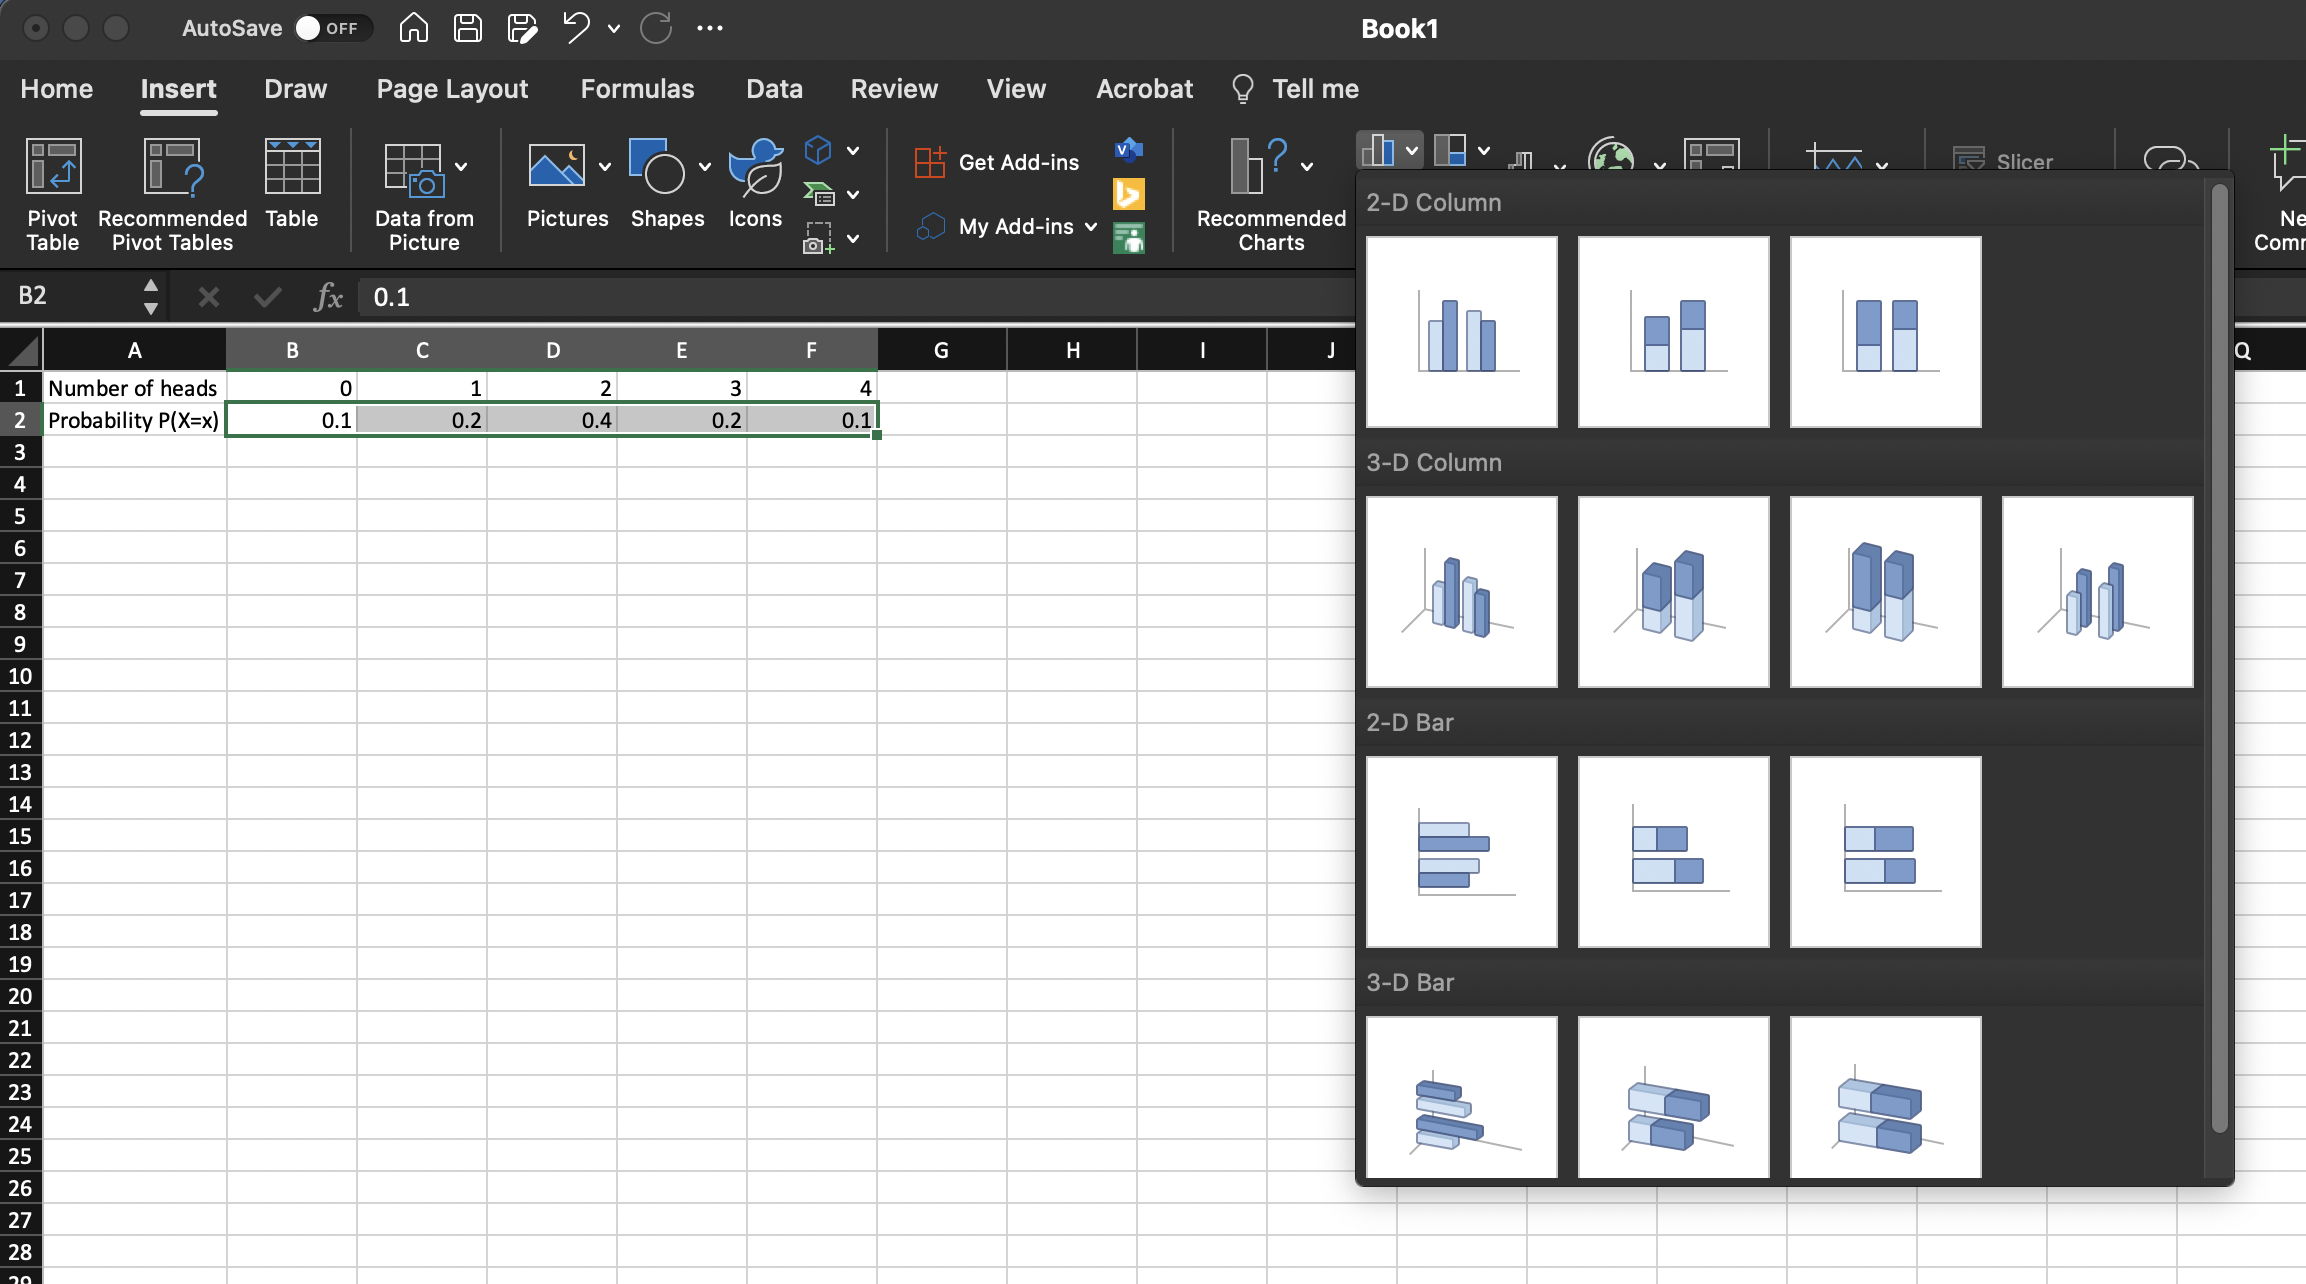
\includegraphics{images/Barchart_1.png}

}

\caption{Barchart 1}

\end{figure}%%
\begin{figure}[H]

{\centering 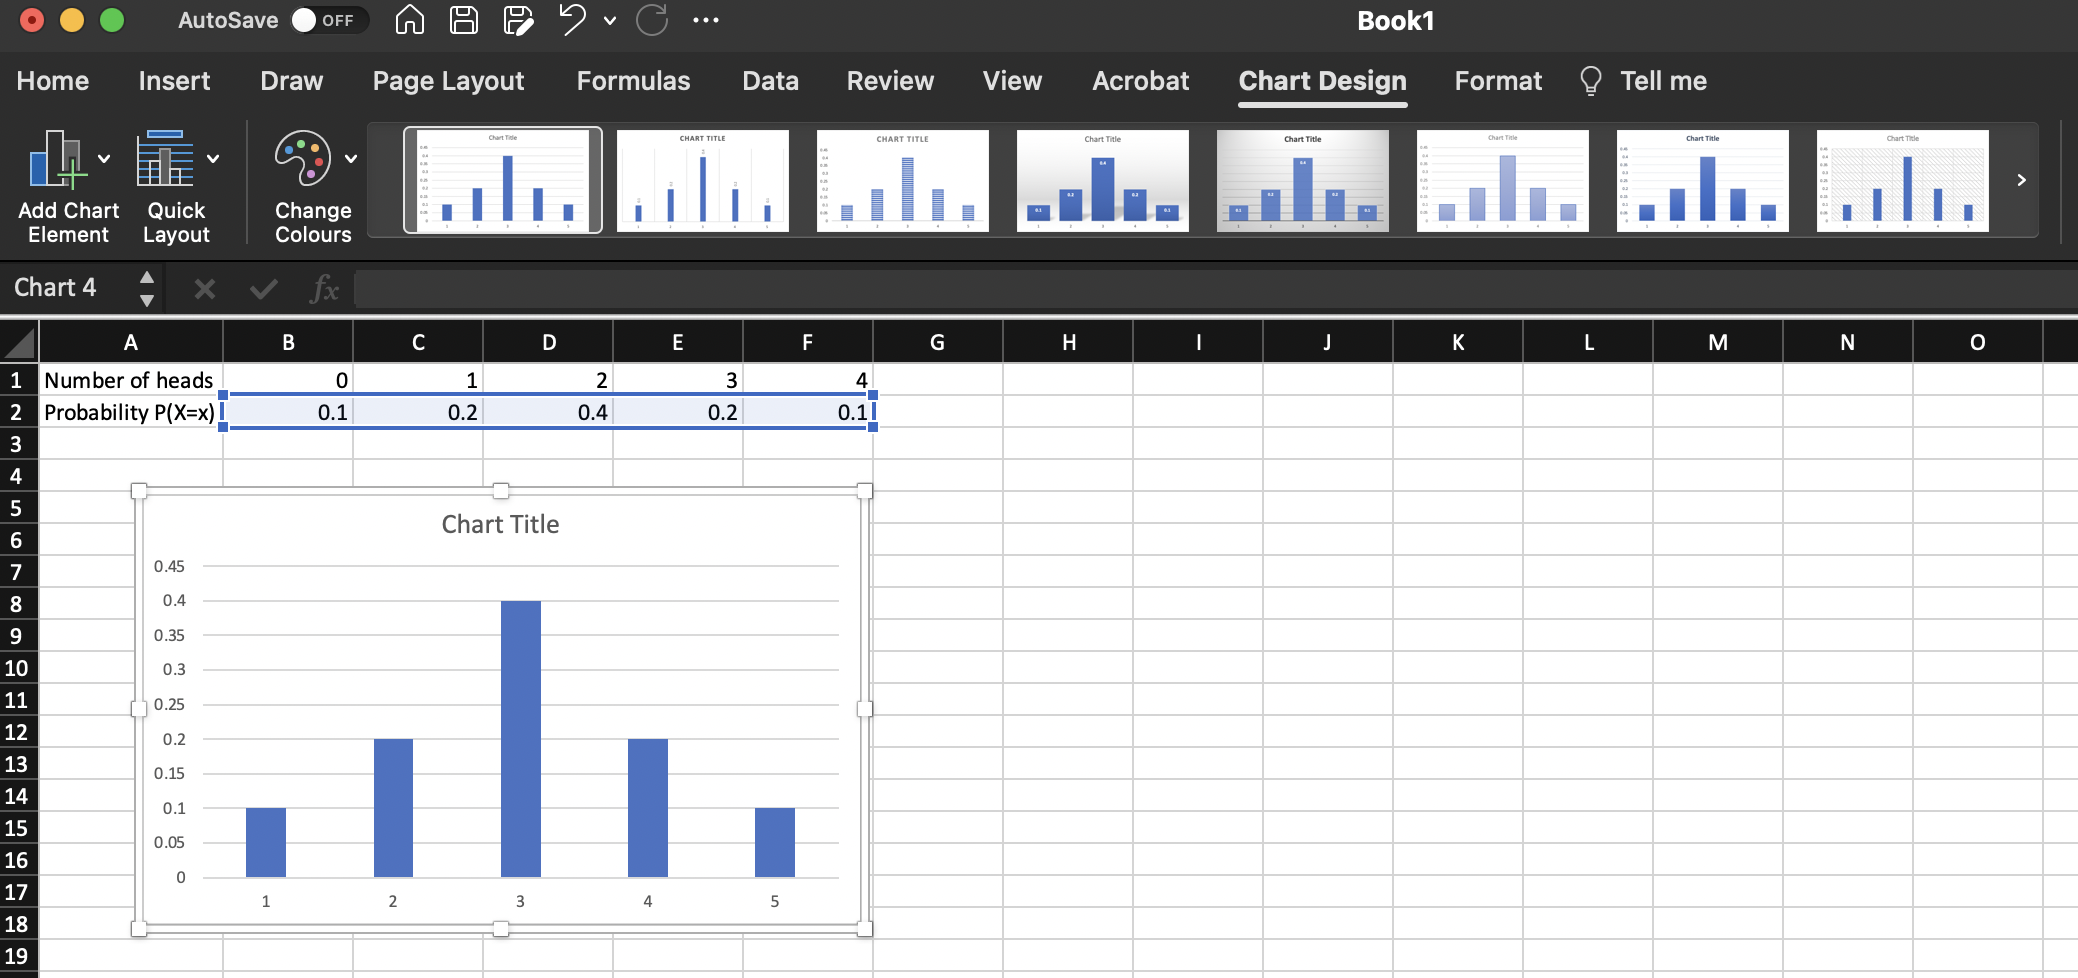
\includegraphics{images/Barchart_2.png}

}

\caption{Barchart 2}

\end{figure}%

\textbf{Question:} With your \textbf{stats} partner, discuss the shape
of the distribution, is it what you would expect to see and compare this
to what the barplot you made in excel, are they similar?

\subsection{Exercise 4}\label{exercise-4}

Now we will use R to simulate 4 coin tosses representing 1 as heads and
0 as tails. Note that I have withheld the output to avoid ``spoiling''
the suprise.

\begin{Shaded}
\begin{Highlighting}[]
\NormalTok{coin }\OtherTok{\textless{}{-}} \FunctionTok{c}\NormalTok{(}\DecValTok{0}\NormalTok{,}\DecValTok{1}\NormalTok{) }\CommentTok{\# vector representing coin tosses c(tails, heads)}
\FunctionTok{set.seed}\NormalTok{(}\DecValTok{1}\NormalTok{) }\CommentTok{\# makes sure we all get the same answer i.e. we use the same randomly generated numbers}
\NormalTok{tosses }\OtherTok{\textless{}{-}} \FunctionTok{sample}\NormalTok{(coin, }\AttributeTok{size =} \DecValTok{4}\SpecialCharTok{*}\DecValTok{20}\NormalTok{, }\AttributeTok{replace =}\NormalTok{ T, }\AttributeTok{prob =} \FunctionTok{c}\NormalTok{(}\FloatTok{0.5}\NormalTok{, }\FloatTok{0.5}\NormalTok{)) }\CommentTok{\# this randomly picks a 0 or 1 from coin and there is an equal probability of sampling both. It creates a vector of results i.e. bo tosses in total}
\FunctionTok{dim}\NormalTok{(tosses) }\OtherTok{\textless{}{-}} \FunctionTok{c}\NormalTok{(}\DecValTok{20}\NormalTok{,}\DecValTok{4}\NormalTok{) }\CommentTok{\# This creates a data frame with 4 columns and 20 rows that represents the 20 trials of 4 coin tosses}
\NormalTok{tosses }\DocumentationTok{\#\# this prints the result}
\NormalTok{NumHeads }\OtherTok{\textless{}{-}} \FunctionTok{rowSums}\NormalTok{(tosses) }\DocumentationTok{\#\# this sums the number of heads in each trial}
\NormalTok{NumHeads }\CommentTok{\# this prints the results  }
\end{Highlighting}
\end{Shaded}

The table function tallies each of the numbers of heads for each
simulation. In each trial (4 tosses) How many times did you toss no
heads, how many times did you toss 1 head, how many times did you toss 2
heads, how many times did you toss 3 heads and how many times did you
toss 4 heads?

\begin{Shaded}
\begin{Highlighting}[]
\NormalTok{Freq\_table }\OtherTok{\textless{}{-}} \FunctionTok{table}\NormalTok{(NumHeads)}
\NormalTok{Freq\_table}
\end{Highlighting}
\end{Shaded}

The prob.table function divides each frequency by 20 i.e.\(P(X=0)=2/20\)

\begin{Shaded}
\begin{Highlighting}[]
\FunctionTok{prop.table}\NormalTok{(Freq\_table) }
\end{Highlighting}
\end{Shaded}

Now we can plot this. Notice how we customise the x-axis to ensure that
0 is displayed as even though there may be no instances where we got
zero heads, it is still a possibility even if the probability is low.
for this we use the argument , xaxt = ``n'' and then draw customised
axis labels using the axis function.

\begin{Shaded}
\begin{Highlighting}[]
\FunctionTok{plot}\NormalTok{(}\FunctionTok{prop.table}\NormalTok{(Freq\_table), }\AttributeTok{ylab=}\StringTok{"P(X=X)"}\NormalTok{, }\AttributeTok{xlab =} \StringTok{"x"}\NormalTok{, }\AttributeTok{xlim =} \FunctionTok{c}\NormalTok{(}\DecValTok{0}\NormalTok{,}\DecValTok{4}\NormalTok{), }\AttributeTok{xaxt =} \StringTok{"n"}\NormalTok{)}
\FunctionTok{axis}\NormalTok{(}\DecValTok{1}\NormalTok{, }\AttributeTok{at =} \DecValTok{0}\SpecialCharTok{:}\DecValTok{4}\NormalTok{)}
\end{Highlighting}
\end{Shaded}

\subsection{Exercise 5}\label{exercise-5}

Repeat exercise 4, but this time change the `prob = c(0.5, 0.5)' to
`prob = c(0.3, 0.7)'.

\textbf{Question:} What happens to the shape of the distribution? What
type of coin does this change in probability represent?

\subsection{Exercise 6}\label{exercise-6}

Repeat exercise 4, but this time change the \texttt{set.seed(1)} to
\texttt{set.seed(123)}.

\textbf{Question:} What happens to the frequency table `Freq\_table' why
do you think it might change?

\subsection{Exercise 7}\label{exercise-7}

Six calves were born after artificial insemination (AI) with regular
semen. Assuming that the probability for either being male or female is
0.5,

\textbf{Question:} What is the probability that all 6 are male?\\

\(X=\) number of male calves \(\sim Bin(n=6,p=0.5)\)
\(P(X=6)=\left(\begin{matrix}6\\6\end{matrix}\right)0.5^6(1-0.5)^{6-6} = 0.015625\)

or in R we can calculate using the dbinom function which calculates the
exact probability of having 6 male calfs born

\begin{Shaded}
\begin{Highlighting}[]
\FunctionTok{dbinom}\NormalTok{(}\DecValTok{6}\NormalTok{,}\DecValTok{6}\NormalTok{,}\FloatTok{0.5}\NormalTok{)}
\end{Highlighting}
\end{Shaded}

\textbf{Question:} What is the probability that more than 4 calves are
female?

NOTE \emph{P(more than 4 calves are female)} = \emph{P(less than 2
calcves are male)} = \emph{P(X=0)+P(X=1)}

\(=\left(\begin{matrix}6\\0\end{matrix}\right)0.5^0(1-0.5)^{6-0}+\left(\begin{matrix}6\\1\end{matrix}\right)0.5^1(1-0.5)^{6-1} = 0.109375\)

or in R

\begin{Shaded}
\begin{Highlighting}[]
\DecValTok{1}\SpecialCharTok{{-}}\FunctionTok{pbinom}\NormalTok{(}\DecValTok{4}\NormalTok{,}\DecValTok{6}\NormalTok{,}\FloatTok{0.5}\NormalTok{)}
\end{Highlighting}
\end{Shaded}

\textbf{Question:} What are your assumptions? What is a more accurate
estimate of the P(male calf)?
https://www.beefmagazine.com/mag/sex\_ratio\_riddle

\textbf{Assumptions:} Each of the births is independent and \emph{P(male
calf = 0.5)}. (In reality, it is 1.06 males per every female born in
large populations of cattle, which gives p = 0.5145631. See article
link.)

Using the updated probability p = 0.5145631 and using R recalculate\\

\textbf{Question:} What is the probability that all 6 are male?\\
\textbf{Question:} What is the probability that more than 4 calves are
female?\\
\textbf{Question:} Finally, calculate what is the probability that
exactly 4 females are born?\\

\section{The Poisson Distribution}\label{the-poisson-distribution}

The Poisson distribution is often used to model the number of expected
events that occur during a given unit of time.

Remember if \(X \sim Po(\lambda)\) then

\(P(X=x)=\frac{\lambda^xe^{-\lambda}}{x!}\) for \(x = 0,1,2,...\) and
\(\lambda>0\)

\subsection{Exercise 1}\label{exercise-1-1}

Lets take a look at an example. Let us assume that \textbf{on average} 5
shoppers enter a store each hour. Say the shop is open for 10 hours per
day, what would a typical day look like. Assuming that the number of
visits follows a Poisson distribution i.e.~If \(X \sim Po(\lambda)\),
and because we know \(\lambda=5\) and \(n=10\), we can simulate this in
R using the following:

\begin{Shaded}
\begin{Highlighting}[]
\NormalTok{shoppers }\OtherTok{\textless{}{-}} \FunctionTok{rpois}\NormalTok{(}\DecValTok{10}\NormalTok{, }\DecValTok{5}\NormalTok{)}
\NormalTok{shoppers}
\end{Highlighting}
\end{Shaded}

\textbf{Question:} Take a look at the minimum and maximum number of
shoppers generated by the model and discuss with your neighbour how you,
as a shop owner, might use this information? \textbf{Question:} Now run
the simulation for a full 5 day week, is there any change?
\textbf{Question:} Now suppose as a shop owner you are concerned that
your shop assistant might get overwhelmed if more than 10 shoppers come
in, in any one hour period, what is the probability of this?

\subsection{Exercise 2}\label{exercise-2-1}

We also often say that the Poisson Distribution is good for modeling
rare events. For example, recent work in Drosophila suggests the
spontaneous rate of deleterious mutations is 1.2 per diploid genome.

Open the following article and read the abstract and then search the
word poisson and read the final two sentences of this paragraph.

http://www.nature.com/nature/journal/v445/n7123/full/nature05388.html

Assume that X = the number of deleterious mutations \(X \sim Po(1.2)\).

\textbf{Question:} What is the probability that an individual has 0
mutations?

\(P(X=0)=\frac{1.2^0e^{-1.2}}{0!}=0.3011942\)

Or in R

\begin{Shaded}
\begin{Highlighting}[]
\FunctionTok{dpois}\NormalTok{(}\DecValTok{0}\NormalTok{,}\FloatTok{1.2}\NormalTok{)}
\end{Highlighting}
\end{Shaded}

\textbf{Question:} What is the probability that an individual has less
than or equal to 2 mutations?

\(P(X\le2)=P(X=0)+P(X=1)+P(X=2)\)
\(=\frac{1.2^0e^{-1.2}}{0!}+\frac{1.2^1e^{-1.2}}{1!}+\frac{1.2^2e^{-1.2}}{2!}\)
\(=0.8794871\)

Or in R

\begin{Shaded}
\begin{Highlighting}[]
\FunctionTok{ppois}\NormalTok{(}\DecValTok{2}\NormalTok{,}\FloatTok{1.2}\NormalTok{)}
\end{Highlighting}
\end{Shaded}

More recent research found that the average spontaneous rate of
deleterious mutations was actually 1.4 per diploid genome. Using R
recalculate the following.\\

\textbf{Question:} What is the new probability that an individual has 0
mutations. How does this compare to the former probability, what does
this suggest?\\
\textbf{Question:} What is the new probability that an individual has
less than or equal to 2 mutations How does this compare to the former
probability, what does this suggest?\\

\subsection{Advanced exercise}\label{advanced-exercise}

From the tutorial we looked at Tomato germination. Use simulations to
find approximate Binomial probabilities obtain an estimate of the
probability of getting 7 or more germinating seeds, by doing simulations
from a \(Bin(8, 0.7)\) in R.

Remember that the exact probability is

\begin{Shaded}
\begin{Highlighting}[]
\DecValTok{1}\SpecialCharTok{{-}}\FunctionTok{pbinom}\NormalTok{(}\DecValTok{6}\NormalTok{,}\DecValTok{8}\NormalTok{,}\FloatTok{0.7}\NormalTok{)}
\end{Highlighting}
\end{Shaded}

\begin{verbatim}
[1] 0.2552983
\end{verbatim}

\begin{itemize}
\tightlist
\item
  First try 10 simulations and fill out a similar table to below in
  excel. What is your estimate of the probability of 7 germinating
  seeds?
\end{itemize}

\begin{Shaded}
\begin{Highlighting}[]
\FunctionTok{set.seed}\NormalTok{(}\DecValTok{123}\NormalTok{)}
\NormalTok{seeds }\OtherTok{\textless{}{-}} \FunctionTok{rbinom}\NormalTok{(}\AttributeTok{n =} \DecValTok{10}\NormalTok{, }\DecValTok{8}\NormalTok{, }\FloatTok{0.7}\NormalTok{) }\CommentTok{\# randomly generates 10 values from Bin(8,0.7)}
\NormalTok{seeds }\DocumentationTok{\#\# prints seeds}
\FunctionTok{table}\NormalTok{(seeds)}\SpecialCharTok{/}\DecValTok{10} \CommentTok{\# turns counts into probabilities}
\FunctionTok{barplot}\NormalTok{(}\FunctionTok{table}\NormalTok{(seeds)}\SpecialCharTok{/}\DecValTok{10}\NormalTok{, }\AttributeTok{xlab=}\StringTok{"Number Germinated x"}\NormalTok{, }\AttributeTok{ylab=}\StringTok{"Probability"}\NormalTok{, }\AttributeTok{col=}\StringTok{"green"}\NormalTok{)}
\end{Highlighting}
\end{Shaded}

\begin{itemize}
\tightlist
\item
  Next try 100 simulations.
\end{itemize}

\begin{Shaded}
\begin{Highlighting}[]
\FunctionTok{set.seed}\NormalTok{(}\DecValTok{123}\NormalTok{)}
\NormalTok{seeds }\OtherTok{\textless{}{-}} \FunctionTok{rbinom}\NormalTok{(}\AttributeTok{n =} \DecValTok{100}\NormalTok{, }\DecValTok{8}\NormalTok{, }\FloatTok{0.7}\NormalTok{) }\CommentTok{\# randomly generates 100 values from Bin(8,0.7)}
\NormalTok{seeds }\DocumentationTok{\#\# prints seeds}
\FunctionTok{table}\NormalTok{(seeds)}\SpecialCharTok{/}\DecValTok{100} \CommentTok{\# turns counts into probabilities}
\FunctionTok{barplot}\NormalTok{(}\FunctionTok{table}\NormalTok{(seeds)}\SpecialCharTok{/}\DecValTok{100}\NormalTok{, }\AttributeTok{xlab=}\StringTok{"Number germinated (x)"}\NormalTok{, }\AttributeTok{ylab=}\StringTok{"Probability"}\NormalTok{, }\AttributeTok{col=}\StringTok{"green"}\NormalTok{)}
\end{Highlighting}
\end{Shaded}

\begin{itemize}
\tightlist
\item
  Now we will try 10000 simulations. What do you notice about the
  histogram?
\end{itemize}

\begin{Shaded}
\begin{Highlighting}[]
\FunctionTok{set.seed}\NormalTok{(}\DecValTok{123}\NormalTok{)}
\NormalTok{seeds }\OtherTok{\textless{}{-}} \FunctionTok{rbinom}\NormalTok{(}\AttributeTok{n =} \DecValTok{10000}\NormalTok{, }\DecValTok{8}\NormalTok{, }\FloatTok{0.7}\NormalTok{) }\CommentTok{\# randomly generates 100 values from Bin(8,0.7)}
\FunctionTok{table}\NormalTok{(seeds)}\SpecialCharTok{/}\DecValTok{10000} \CommentTok{\# turns counts into probabilities}
\FunctionTok{barplot}\NormalTok{(}\FunctionTok{table}\NormalTok{(seeds)}\SpecialCharTok{/}\DecValTok{10000}\NormalTok{, }\AttributeTok{xlab=}\StringTok{"Number germinated (x)"}\NormalTok{, }\AttributeTok{ylab=}\StringTok{"Probability"}\NormalTok{, }\AttributeTok{col=}\StringTok{"green"}\NormalTok{)}
\end{Highlighting}
\end{Shaded}

\begin{enumerate}
\def\labelenumi{\arabic{enumi}.}
\setcounter{enumi}{4}
\tightlist
\item
  Now we can compare the exact results and the simulated results by
  adding up the probabilities for 7 and 8 seeds germinating in each of
  the scenarios.
\end{enumerate}

\textbf{Note} that the numbers will may differ slightly each time as
they a randomly generated unless you set the same seed.

\begin{longtable}[]{@{}ll@{}}
\toprule\noalign{}
Number germinated & \(P(X\ge{7}\)) \\
\midrule\noalign{}
\endhead
\bottomrule\noalign{}
\endlastfoot
Exact method using R & \\
Simulation (n=10) & \\
Simulation (n=100) & \\
Simulation (n=10000) & \\
\end{longtable}

\textbf{Question:} Which of the simulations gives the closest result to
the exact method, why do you think this is - try ask chatGPT?



\end{document}
